% \section{Vorstellung der Demoanwendung}

Vor dem zu erstellenden Konzept wird zunächst eine Demoanwendung erstellt, an der das Konzept anzuwenden ist. Dieser Abschnitt beschäftigt sich mit der Vorstellung der Demoanwendung, wie diese aufgebaut ist und was für eine Art von Webanwendung sie repräsentiert.

Die Motivation nennt ein konkretes Problem eines Kunden der Open Knowledge. Um eine moderne Webanwendung \cite{RichWebBasedApplications} darzustellen, wird die Demoanwendung in Grundzügen den Aufbau der Webanwendung des Direktversicherers nachahmen. Die Webanwendung realisiert einen Wizard \cite{EzMolAWebServerWizard}, also eine Sequenz von aufeinanderfolgenden Dialogseiten bei dem der Nutzer Daten eingeben soll. Bei der Webanwendung handelt es sich um eine clientbasierte Angular-SPA. Die Webanwendung validiert einzelne Felder gegen Partnersysteme (bspw. beim Adressfeld). Am Ende des Wizards werden die gesamten Daten an ein weiteres Partnersystem übermittelt, welches darauf basierend eine Berechnung durchführt und das Ergebnis dann an die Webanwendung sendet.

Die Demoanwendung soll eine Bestellfunktionalität eines Obst-Webshops darstellen. Der Warenkorb hierfür wird anfangs dynamisch generiert und simuliert so, dass dieser durch einen vorgelagerten Prozess erstellt wurde. Der Nutzer soll seine Rechnungs- und Lieferdaten eingeben und am Ende die Bestellung ausführen können. Um das gewünschte Verhalten der Demoanwendung zu definieren, wird es im folgenden Abschnitt festgelegt.

\subsection{Verhaltensdefinition}

Der gewünschte Funktionsumfang der Demoanwendung wurde mittels einer Verhaltensdefinition festgehalten. Diesen Ansatz der Definition der Software anhand des Verhaltens nennt man Behavior-Driven Development (BDD). BDD wurde 2006 erstmals von Dan North benannt und definiert \cite{IntroducingBDD}. Bei BDD werden User-Stories aus der Sicht eines äußerlichen Betrachters entworfen und geschrieben. Dabei umfassen die User-Stories Beispiele, wie sich die Anwendung in diesen Szenarien verhalten soll.

Die BDD-Definition wurde in der gängigen Gherkin-Syntax \cite{Gherkin} geschrieben. Die Syntax ist natürlich zu lesen. Nachfolgend werden alle gewünschten Features der Demoanwendung in der Gherkin-Syntax aufgelistet.

\lstinputlisting[
  language = gherkin,
   caption = Demoanwendung: Gherkin Definition zum Feature \enquote{Warenkorb},
captionpos = b,
     label = lst:demoanwendung-gherkin-warenkorb
]{content/04_erstellung-poc/warenkorb-gherkin/1-warenkorb.feature}

\lstinputlisting[
  language = gherkin,
   caption = Demoanwendung: Gherkin Definition zum Feature \enquote{Rechnungsadresse},
captionpos = b,
     label = lst:demoanwendung-gherkin-rechnungsadresse
]{content/04_erstellung-poc/warenkorb-gherkin/2-rechnungsadresse.feature}

\lstinputlisting[
  language = gherkin,
   caption = Demoanwendung: Gherkin Definition zum Feature \enquote{Lieferadresse},
captionpos = b,
     label = lst:demoanwendung-gherkin-lieferadresse
]{content/04_erstellung-poc/warenkorb-gherkin/3-lieferadresse.feature}

\lstinputlisting[
  language = gherkin,
   caption = Demoanwendung: Gherkin Definition zum Feature \enquote{Zahlungsdaten},
captionpos = b,
     label = lst:demoanwendung-gherkin-zahlungsdaten
]{content/04_erstellung-poc/warenkorb-gherkin/4-zahlungsdaten.feature}

\lstinputlisting[
  language = gherkin,
   caption = Demoanwendung: Gherkin Definition zum Feature \enquote{Bestellung abschließen},
captionpos = b,
     label = lst:demoanwendung-gherkin-bestellung_abschließen
]{content/04_erstellung-poc/warenkorb-gherkin/5-bestellung_abschließen.feature}

Neben dem Frontend soll ein dazugehöriges Backend Teil der Demoanwendung sein. Auf Basis der Verhaltensdefinition wurde eine Architektur entworfen, welche im folgenden Abschnitt näher erläutert wird.

\subsection{Backend}
\label{subsec:demoanwendung-backend}

Das Backend wurde als Microservice-Architektur \cite{MicroserviceArchitecture} konzipiert und orientiert sich grob an der Architektur, die der Direktversicherer derzeit betreibt. Die einzelnen Dienste wurden auf Basis von Java EE sowie Kubernetes erstellt. In \autoref{fig:demoanwendung_deployment} lässt sich die Architektur betrachten, hierbei stellen Pods einzelne Containersysteme dar.

Die Kommunikation mit dem Backend erfolgt über einen Service, der das \enquote{Backend\-4\-Frontend}-Pattern realisiert. Das Backend4Frontend bündelt alle Schnittstellen der dahinter liegenden Dienste, sodass das Frontend nur mit einem einzelnen Dienst kommunizieren muss. Die weiteren Dienste \enquote{Bestellungen}, \enquote{Übersetzungen}, \enquote{Addressvalidierung} und \enquote{Warenkorb} übernehmen die jeweilige Funktion, die ihr Name beschreibt. Der Dienst \enquote{Bestellungen} ist das Partnersystem, welches beim Fertigstellen des Wizards aufgerufen wird und es führt dabei weitere Datenabfragen und Validitätsüberprüfungen mit Partnerdiensten durch.

\begin{figure}[H]
	\centering
	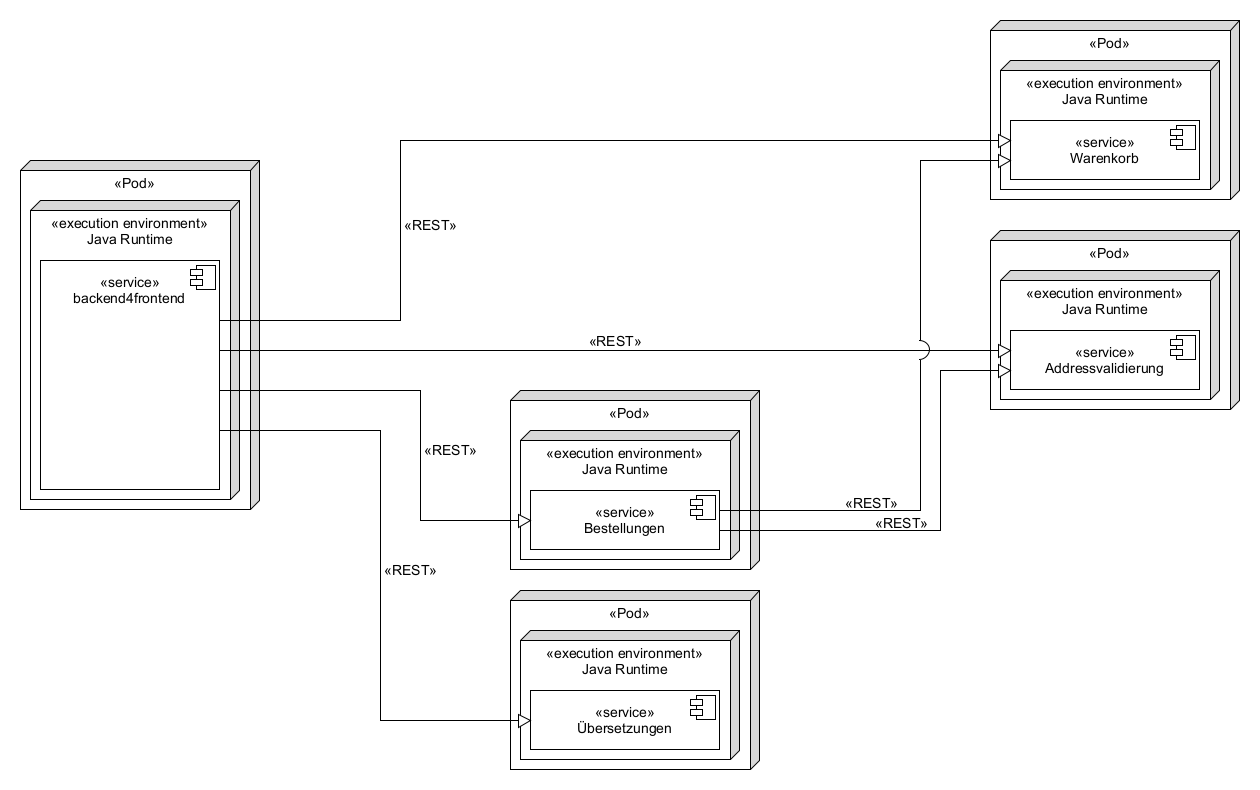
\includegraphics[width=1.00\linewidth]{img/04_erstellung-poc/demoanwendung_deployment.png}
	\caption{Demoanwendung: Deployment-Diagramm. Eigene Darstellung}
	\label{fig:demoanwendung_deployment}
\end{figure}

Die einzelnen Dienste wurden mit Eclipse MicroProfile \cite{EclipseMicroprofile} umgesetzt. MicroProfile ist eine Sammlung verschiedener Java-EE-Frameworks und Technologien zur Umsetzung von Microservices. Kern der Dienste, die auf MicroProfile basieren, sind die REST-Schnittstellen, die mit JAX-RS umgesetzt werden.

Die einzelnen Dienste wurden jeweils als Docker-Images\footnote{Docker \cite{Docker} ist eine Software zum Erstellen und Ausführen von Anwendungscontainern \cite{PatternsForSoftwareOrchestration}} gepackt, zur Gewährleistung einer einheitlichen Umgebung auch auf unterschiedlichen Rechnern. Um ein einfaches Management der Services zu ermöglichen, wird die Plattform Kubernetes\footnote{Kubernetes \cite{Kubernetes} ist eine Software zum Orchestrieren Container-basierter Anwendungen \cite{KeyCharacteristicsOfAContainerOrchestrationPlatform}} verwendet.

\subsection{Frontend}

Auf Basis von Angular realisiert das Frontend einen Wizard, welcher mehrere aufeinander folgende Formulare in derselben SPA enthält. Anhand des folgenden Durchlaufs werden die einzelnen Seiten des Frontends beispielhaft veranschaulicht:

\begin{quotation}
	\begin{flushleft}
		Warenkorb \textrightarrow{} Rechnungsadresse  \textrightarrow{} Lieferdaten \textrightarrow{} Zahlungsdaten
	\par{}
	\end{flushleft}
	\begin{flushright}
		 \textrightarrow{} Bestellung abschließen \textrightarrow{} Bestellbestätigung
	\end{flushright}
\end{quotation}

\subsubsection{Warenkorb}

Die erste Seite des Wizards zeigt den Inhalt des Warenkorbs eines Online-Shops für Früchte (vgl \autoref{fig:demoanwendung_vorstellung_01-warenkorb}). Hier kann der Nutzer seine Auswahl prüfen und bei Zufriedenheit kann er den Bestellvorgang starten.

Die hier angezeigten Daten werden vom Warenkorbdienst abgerufen, über die Angabe eines zuvor zufällig generierten Warenkorb-Identifiers. Die Warenkorbdaten werden zudem mit Übersetzungsdaten vom Übersetzungsdienst angereichert, denn in den Warenkorbdaten stehen lediglich Übersetzungsschlüssel wie \texttt{item.peach}, die dann auf den tatsächlichen Übersetzungswert abgebildet werden also \texttt{Pfirsich}. Beim Starten des Bestellvorgangs wird kein Serverabruf durchgeführt, sondern in der SPA wird ein Seitenwechsel vorgenommen.

\begin{figure}[H]
	\centering
	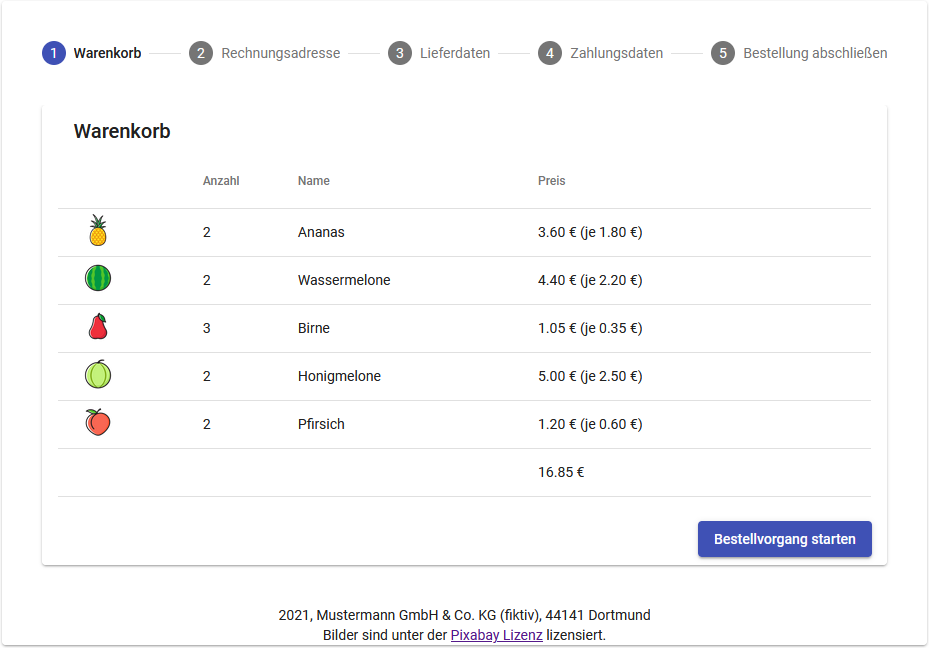
\includegraphics[width=1.00\linewidth]{img/04_erstellung-poc/demoanwendung_vorstellung_01-warenkorb_more-items.png}
	\caption{Demoanwendung: Startseite \enquote{Warenkorb}. Eigener Screenshot}
	\label{fig:demoanwendung_vorstellung_01-warenkorb}
\end{figure}

\subsubsection{Rechnungsadresse}

Auf der zweiten Seite des Wizards wird die Rechnungsadresse erfasst (vgl. \autoref{fig:demoanwendung_vorstellung_02-rechnungsadresse}). Hierbei wird der Nutzer gebeten rechnungsrelevante Informationen, wie seine Adresse, anzugeben. Er kann jedoch auch auf die vorherige Seite zurückspringen.

Beim Absenden des Formulars wird zunächst die Validität der Eingabefelder überprüft, bspw. ob die PLZ aus 5 Zahlen besteht, und anschließend wird die Adresse dem Adressvalidierungsdienst zur Prüfung übergeben. Schlägt eine Validierung fehl, so wird dies entweder direkt am verursachenden Textfeld angezeigt oder in einer allgemeinen Fehlermeldung im unteren Bereich der Eingabemaske ausgegeben.

Sind beide Prüfungen jedoch erfolgreich, so wird ein Seitenwechsel in der SPA durchgeführt. Neben der Adressüberprüfung wird kein zusätzlicher Serveraufruf abgesetzt, die eingegeben Daten werden jedoch intern einer übergeordneten Komponente übergeben.

\begin{figure}[H]
	\centering
	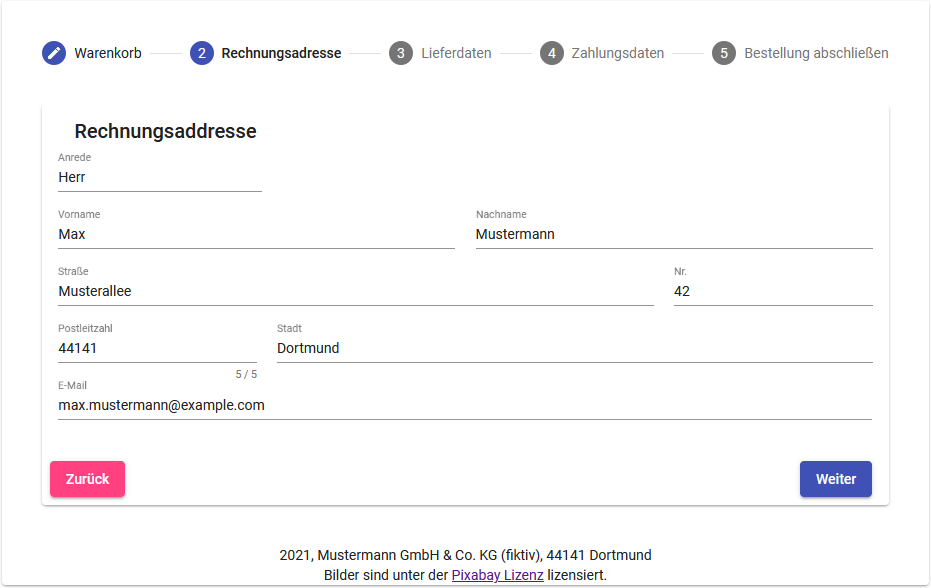
\includegraphics[width=1.00\linewidth]{img/04_erstellung-poc/demoanwendung_vorstellung_02-rechnungsadresse.png}
	\caption{Demoanwendung: Seite \enquote{Rechnungsadresse}. Eigener Screenshot}
	\label{fig:demoanwendung_vorstellung_02-rechnungsadresse}
\end{figure}

\newpage

\subsubsection{Lieferdaten}

Die dritte Seite des Wizards erfasst die Lieferdaten des Nutzers. Der Nutzer kann entweder die relevanten Daten aus der Rechnungsadresse übernehmen lassen (Standardfall) oder er gibt alternativ abweichende Lieferdaten an, wie in \autoref{fig:demoanwendung_vorstellung_03-lieferdaten} zu sehen ist. Wie zuvor kann der Nutzer auch auf das vorherige Formular zurückspringen.

Bei der Angabe von abweichenden Lieferdaten werden, wie beim Formular der Rechnungsadresse, zunächst die Eingabefelder überprüft und bei Fehlschlag visuell dem Nutzer kenntlich gemacht. Anders als bei der Rechnungsadresse wird jedoch nicht der Adressvalidierungsdienst befragt, dies wird im \autoref{subsec:ungueltige-adressen-sind-gueltig} aufgefasst und erläutert.

Sind keine abweichenden Lieferdaten erwünscht oder die Validierung der Eingaben erfolgt, wird beim Klick auf \enquote{Weiter} ein Seitenwechsel in der SPA durchgeführt. Auch hier erfolgt kein Serveraufruf, jedoch werden die Daten an die übergeordnete Komponente innerhalb der Webanwendung weitergereicht.

\begin{figure}[H]
	\centering
	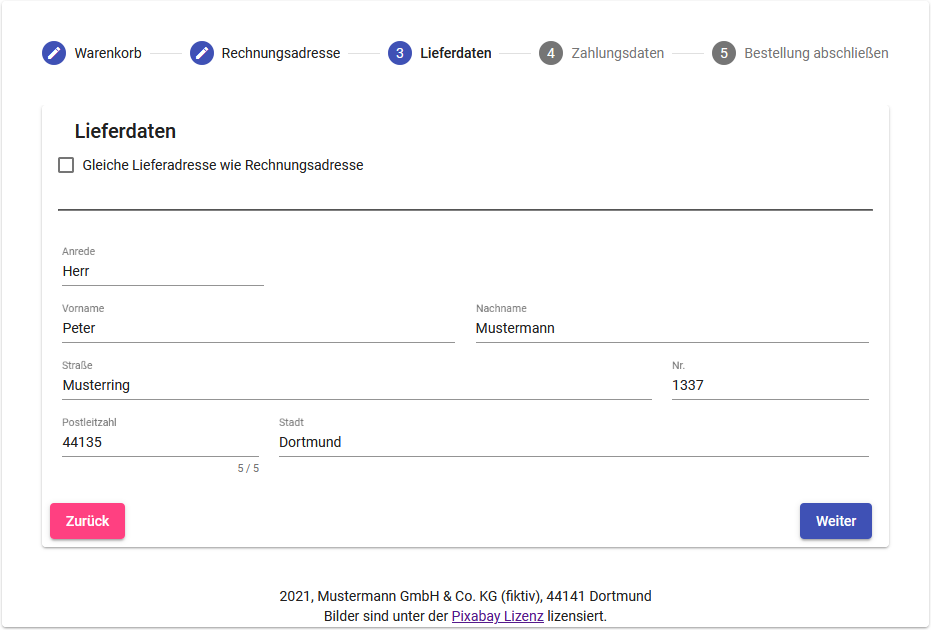
\includegraphics[width=1.00\linewidth]{img/04_erstellung-poc/demoanwendung_vorstellung_03-lieferdaten.png}
	\caption{Demoanwendung: Seite \enquote{Lieferdaten}. Eigener Screenshot}
	\label{fig:demoanwendung_vorstellung_03-lieferdaten}
\end{figure}

\subsubsection{Zahlungsdaten}

Die vierte Seite des Wizards bittet den Nutzer zur Eingabe seiner gewünschten Zahlart sowie der jew. Zahlungsinformationen. Dabei kann der er zwischen 4 Zahlungsarten wählen: per Rechnung, Lastschrift, PayPal oder Kreditkarte. Wie bei den anderen Formularen kann der Nutzer auf das vorhergehende Formular über den Button \enquote{Zurück} wechseln.

Bei Auswahl der Rechnungsart \enquote{Rechnung} muss der Nutzer keine weiteren Daten eingeben. Hingegen sind bei anderen Rechnungsarten weitere Daten einzugeben, wie z. B. der in der \autoref{fig:demoanwendung_vorstellung_04-zahlungsdaten} zu betrachteter Rechnungsart \enquote{Lastschrift}, hier muss der Kontoinhaber und die IBAN angegeben werden. Bei PayPal ist die E-Mail anzugeben und bei der Auswahl der Kreditkarte folgende Kreditkarteninformationen: Karteninhaber, Kartennummer, CVC sowie das Ablaufdatum. Die jeweilig einzugebenden Daten werden clientseitig validiert, ähnlich wie bei den vorherigen Formularen.

Ist eine Rechnungsart ausgewählt und die einzugebenden Daten valide ausgefüllt, so führt ein Absenden des Formulars zu einem Seitenwechsel auf die Seite zum Abschließen der Bestellung. Es wird keine zusätzliche Serverinteraktion durchgeführt, die Daten werden jedoch erneut an die übergeordnete Komponente übergeben.

\begin{figure}[H]
	\centering
	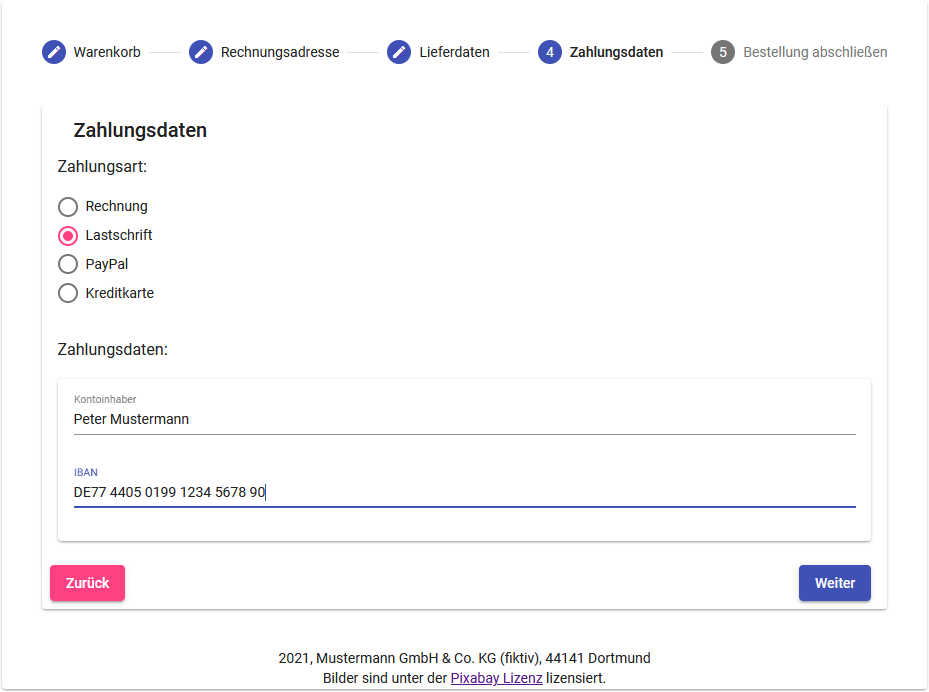
\includegraphics[width=0.85\linewidth]{img/04_erstellung-poc/demoanwendung_vorstellung_04-zahlungsdaten.png}
	\caption{Demoanwendung: Seite \enquote{Zahlungsdaten}. Eigener Screenshot}
	\label{fig:demoanwendung_vorstellung_04-zahlungsdaten}
\end{figure}

\subsubsection{Bestellübersicht}

Die vorletzte Seite des Wizard fasst die Bestelldaten zusammen (vgl. \autoref{fig:demoanwendung_vorstellung_05-bestelluebersicht}) und sendet die Daten bei der Bestätigung des Formulars an das Backend. Wie bei allen Formularen gibt es auch hier die Option für den Nutzer zu einem vorherigen Formular zurückzuspringen und Anpassungen vorzunehmen.

In der Bestellübersicht werden explizit der ausgewählte Warenkorb, die eingegebenen Rechnungs- und Lieferadresse sowie die gewählte Zahlungsart dargestellt. Der Warenkorb wird hierbei analog zur Warenkorbseite vom Warenkorbdienst abgefragt. Zuvor eingegebene Daten sind hingegen lediglich clientseitig gespeichert und werden von einer übergreifenden Komponente bereitgestellt. Weitere Eingaben des Nutzers sind auf dieser Seite aber nicht gefordert, sie dient hauptsächlich der visuellen Überprüfung für den Nutzer, bevor er die Bestellung kostenpflichtig durchführt.

Sendet der Nutzer die Bestellung ab, werden die zuvor eingegeben Daten und der Identifier des Warenkorbs an den Bestelldienst übergeben. Dieser überprüft beide Adresseingaben gegen den Adressvalidierungsdienst, ruft den Warenkorb vom Warenkorbdienst ab und errechnet auf dieser Datenbasis den Bestellbeleg. Der Bestellbeleg wird dem Frontend in der Antwort übergeben, weiterhin erfolgt ein Seitenwechsel.

\begin{figure}[H]
	\centering
	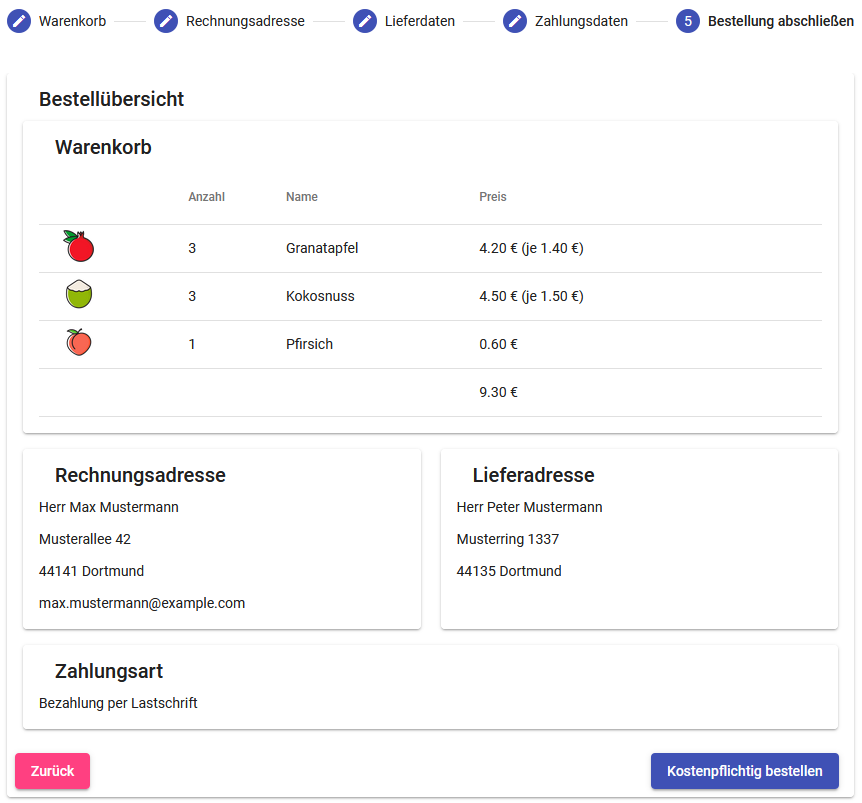
\includegraphics[width=0.68\linewidth]{img/04_erstellung-poc/demoanwendung_vorstellung_05-bestelluebersicht_cropped}
	\caption{Demoanwendung: Seite \enquote{Bestellübersicht}. Eigener Screenshot}
	\label{fig:demoanwendung_vorstellung_05-bestelluebersicht}
\end{figure}

\subsubsection{Bestellbestätigung}

Die sechste und letzte Seite des Wizards visualisiert die Bestellbestätigung nach einer erfolgreichen Bestellung, wie in \autoref{fig:demoanwendung_vorstellung_06-bestellbestaetigung} zu sehen ist. Bei den angezeigten Daten handelt es sich nicht um die zuvor gespeicherten, sondern ausschließlich um die vom Bestelldienst übermittelten Daten.

Auf dieser Seite kann der Nutzer nun nur noch auf den Button \enquote{Zum Shop} klicken und gelangt erneut zur Startseite, jedoch mit einem neuen Warenkorb.

\begin{figure}[H]
	\centering
	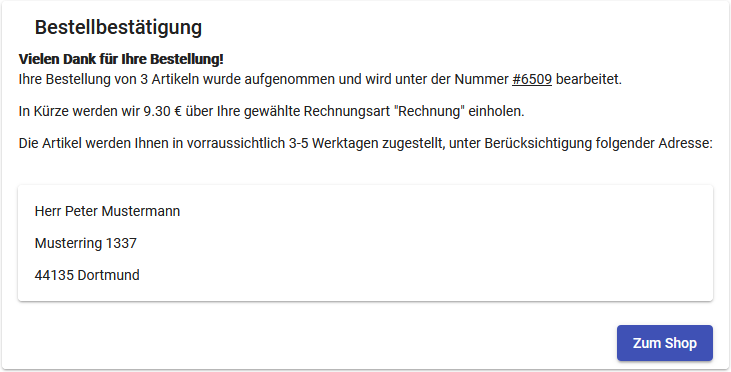
\includegraphics[width=0.75\linewidth]{img/04_erstellung-poc/demoanwendung_vorstellung_06-bestellbestaetigung.png}
	\caption{Demoanwendung: Finale Seite \enquote{Bestellbestätigung}. Eigener Screenshot}
	\label{fig:demoanwendung_vorstellung_06-bestellbestaetigung}
\end{figure}

\subsection{Fehlerszenarien}
\label{subsec:fehlerszenarien}

Um später mithilfe von Observability-Werkzeugen Probleme aufzudecken und Aspekte der Nachvollziehbarkeit darzustellen, weist die Demoanwendung eine Reihe von typischen Fehlern auf, die bewusst integriert wurden.

Diese Fehler gehören unterschiedlichen Problemgruppen an, sie reichen von unerwünscht strenger Validierung, über Konfigurationsfehlern bis hin zu ineffizienter Datenverarbeitung. Ein Ausschnitt wird folgend in Fehlerszenarien beschrieben, aus der Sicht eines Projektteams, welches diese Szenarien berichtet bekommen oder selbst notiert hat.

\pagebreak

\subsubsection{\enquote{Keine Übersetzungen}}
\label{subsec:keine-uebersetzungen}

\begin{wrapfigure}[7]{r}{0.33\textwidth}
\centering
\vspace{-\baselineskip}
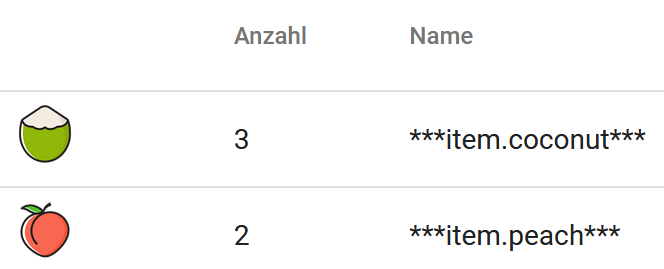
\includegraphics[width=\linewidth]{img/04_erstellung-poc/demoanwendung_fehlerszenario-uebersetzungen}
\caption{Fehlende Texte. Eigener Screenshot}
\label{fig:demoanwendung_fehlerszenario-uebersetzungen}
\end{wrapfigure}

- Problem: Nutzer berichten, dass manchmal die Webanwendung beim Start keine Artikeltexte anzeigt (vgl \autoref{fig:demoanwendung_fehlerszenario-uebersetzungen}).

- Ursache: Die Pods, die den Übersetzungsdienst enthalten, werden repliziert bereitgestellt. Einer der Pods hat eine defekte Konfiguration, weswegen er keine Übersetzungen der Artikel enthält. Wird zu diesem Pod verbunden, tritt das Fehlverhalten auf. Dies ist eine Nachstellung eines tatsächlichen Problems beim Kunden.

%\subsubsection{\enquote{Gültige Straßen sind ungültig}}
%
%- Problem: Nutzer berichten, dass Ihr Straßenname nicht eingeben werden kann. Beispielsweise führt die Eingabe \enquote{Ährenweg} zu einem Fehler.
%
%- Ursache: Der Adressvalidierungsdienst validiert Straßen mit dem Regular-Expression \texttt{[a-zA-Z\textbackslash,\textbackslash-\textbackslash ]+}, welches keine gängigen Sonderzeichen (ä ,ö ,ü, ß) erlaubt.

% rausgenommen, zu viel Dopplung
%\subsubsection{\enquote{Gültige Hausnummern sind ungültig}}
%
%- Problem: Nutzer berichten, dass Hausnummern, die nicht nur aus Zahlen bestehen, zum Fehler führen.
%
%- Ursache: Der Adressvalidierungsdienst validiert Hausnummern als Zahl und schlägt im o. g. Fall in der Konvertierung fehl.

%\subsubsection{\enquote{Gültige Städte sind ungültig}}
%
%- Problem: Nutzer aus Gießen berichten, dass Sie das Formular zur Rechnungsadresse nicht ausfüllen können
%
%- Ursache: Der Adressvalidierungsdienst meldet die Stadt \enquote{Gießen} als ungültig, weil sie nicht in der lokalen Tabelle vorhanden ist.

\subsubsection{\enquote{Ungültige Adressen sind gültig}}
\label{subsec:ungueltige-adressen-sind-gueltig}

- Problem: Nutzer können in den Lieferdaten ungültige Eingaben tätigen und absenden, bei der Bestellaufgabe kommt es zu einem Fehler.

- Ursache: Das Frontend überprüft lediglich die Rechnungsadresse, aber nicht die Lieferadresse

%\subsubsection{\enquote{Vor- und Nachnamen werden abgeschnitten}}
%
%- Problem: Nutzer berichten, dass in der Bestellbestätigung Ihre Vor- und Nachnamen abgeschnitten dargestellt werden.
%
%- Ursache: Der Bestelldienst begrenzt den Vor- sowie den Nachnamen auf 20 Zeichen, das Frontend begrenzt dies jedoch nicht.

%\subsubsection{\enquote{Falsche Zahlungsart}}
%
%- Problem: Nutzer berichten, dass in der Bestellbestätigung die falsche Zahlungsart angezeigt wird. In der Bestellübersicht wurde jedoch die korrekte Zahlungsart angezeigt.
%
%- Ursache: Das Frontend sendet alle Formulardaten jeder Rechnungsart an den Dienst \enquote{Bestellungen}. Dieser nimmt aber an, dass alle nicht ausgewählten Rechnungsarten statt Formulardaten nur \texttt{null} enthalten.

\subsubsection{\enquote{Lange Verarbeitung}}
\label{subsec:lange-verarbeitung}

- Problem: Beim Abrufen der Warenkorbdaten kommt es zu einer unerwünschten Wartezeit (von ca. 6-10s).

- Ursache: Dies ist eine simulierte Wartezeit im Frontend, hierbei wird eine ineffiziente Mapping-Operation nachgeahmt.

%\subsection{Repräsentation}
%
%Eine wichtige Eigenschaft der Demoanwendung sollte sein, dass sie repräsentativ für die Webanwendung des Kunden ist und im Allgemeineren auch für moderne Webanwendungen ist. Durch den groben Aufbau der Demoanwendung, also einer zustandsreichen und zu großen Teilen clientbasierten SPA, stellt die Demoanwendung eine moderne Webanwendung dar. Auch die Verwendung von Angular ist repräsentativ, denn Angular ist eines der meist verwendeten Frontend-Frameworks \cite{TheStateOfJavaScript2020}.
%
%Das Backend ist in dem Sinne repräsentativ, dass es auf keiner stark vereinfachten Infrastruktur basiert, sondern gewollt an die Situation des Open Knowledge Kunden abbildet. Des Weiteren stellt die gewählte Architektur einen modernen Ansatz dar, denn die Architektur ist Microservice-orientiert \cite{MicroserviceArchitecture}.

\subsection{Repräsentation}

Es ist anzumerken, dass die Demoanwendung nur ein Modell einer tatsächlichen Webanwendung darstellt. Wie jedes Modell können nicht alle Gegebenheiten des zu modellierenden Sachverhalts nachgestellt werden. Jedoch ist durch den allgemein gehaltenen Anwendungsfall und die moderne Umsetzung eine Übertragbarkeit zu ähnlichen Projekten durchaus vorhanden.

Nun da die Demoanwendung beschrieben ist, werden die Anforderungen näher erläutert, die das zu erstellende Proof-of-Concept erfüllen soll.

\pagebreak